\documentclass{standalone}
\usepackage{pgfplots}
\pgfplotsset{compat=1.18}

\begin{document}

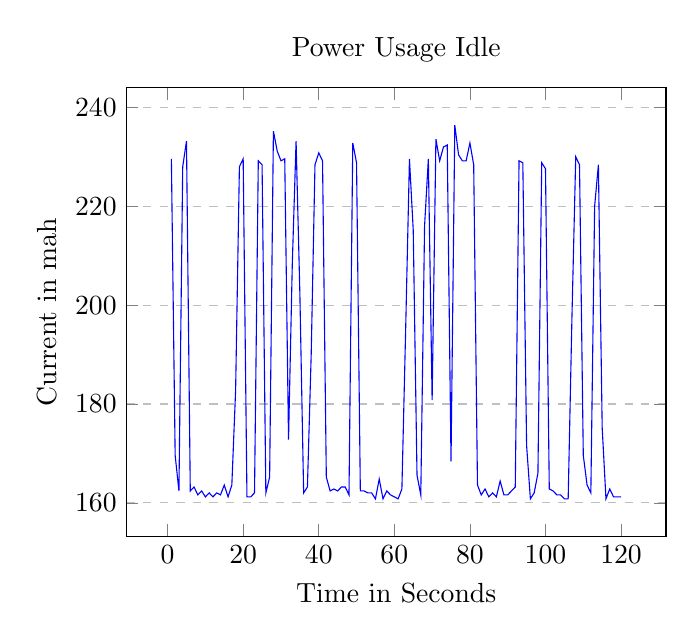
\begin{tikzpicture}
    \begin{axis}[
    title={Power Usage Idle},
    xlabel={Time in Seconds},
    ylabel={Current in mah},
    %ytick=data,
    %xtick=data,
    ymajorgrids=true,
    legend pos=outer north east,
    grid style=dashed,
    ]
    \addplot[
        color=blue,
    ]
    coordinates {
        (1,229.60)
        (2,169.60)
        (3,162.40)
        (4,228.00)
        (5,233.20)
        (6,162.40)
        (7,163.20)
        (8,161.60)
        (9,162.40)
        (10,161.20)
        (11,162.00)
        (12,161.20)
        (13,162.00)
        (14,161.60)
        (15,163.60)
        (16,161.20)
        (17,163.60)
        (18,182.80)
        (19,228.00)
        (20,229.60)
        (21,161.20)
        (22,161.20)
        (23,162.00)
        (24,229.20)
        (25,228.40)
        (26,162.00)
        (27,165.20)
        (28,235.20)
        (29,231.20)
        (30,229.20)
        (31,229.60)
        (32,172.80)
        (33,208.40)
        (34,233.20)
        (35,202.40)
        (36,162.00)
        (37,163.20)
        (38,190.00)
        (39,228.40)
        (40,230.80)
        (41,229.20)
        (42,165.20)
        (43,162.40)
        (44,162.80)
        (45,162.40)
        (46,163.20)
        (47,163.20)
        (48,161.60)
        (49,232.80)
        (50,228.80)
        (51,162.40)
        (52,162.40)
        (53,162.00)
        (54,162.00)
        (55,160.80)
        (56,164.80)
        (57,160.80)
        (58,162.40)
        (59,161.60)
        (60,161.20)
        (61,160.80)
        (62,162.80)
        (63,195.20)
        (64,229.60)
        (65,215.20)
        (66,165.60)
        (67,161.60)
        (68,216.00)
        (69,229.60)
        (70,180.80)
        (71,233.60)
        (72,229.20)
        (73,232.00)
        (74,232.40)
        (75,168.40)
        (76,236.40)
        (77,230.40)
        (78,229.20)
        (79,229.20)
        (80,232.80)
        (81,228.40)
        (82,163.60)
        (83,161.60)
        (84,162.80)
        (85,161.20)
        (86,162.00)
        (87,161.20)
        (88,164.40)
        (89,161.60)
        (90,161.60)
        (91,162.40)
        (92,163.20)
        (93,229.20)
        (94,228.80)
        (95,171.60)
        (96,160.80)
        (97,162.00)
        (98,166.00)
        (99,228.80)
        (100,227.60)
        (101,162.80)
        (102,162.40)
        (103,161.60)
        (104,161.60)
        (105,160.80)
        (106,160.80)
        (107,197.60)
        (108,230.00)
        (109,228.40)
        (110,169.60)
        (111,163.60)
        (112,162.00)
        (113,220.00)
        (114,228.40)
        (115,175.20)
        (116,160.80)
        (117,162.80)
        (118,161.20)
        (119,161.20)
        (120,161.20)
    };
    \end{axis}
\end{tikzpicture}
mean: 186.32
\end{document}
